\chapter{Marco Teórico}

El presente capítulo está orientado a describir conceptos importantes para comprender el funcionamiento de los procesos de trabajo de un estudio de tatuajes profesional. Además, se darán a conocer las tecnologías que serán parte del proyecto y las metodologías que se usarán para ejecutar y evaluar los resultados del mismo.

\section{Plataformas digitales}

Para abordar las necesidades identificadas del cliente experto, se propone el desarrollo de una plataforma digital integral que unifique las funciones operativas y administrativas del estudio de tatuajes. Para ello se evaluaron diferentes alternativas tecnológicas con el fin de seleccionar una solución que permita centralizar el flujo de trabajo, optimizar la gestión de citas, automatizar las cotizaciones y facilitar la previsualización de diseños. A continuación, se presentan las principales características, ventajas y limitaciones de cada enfoque, junto con una comparación basada en dimensiones críticas para el proyecto.

\vspace{\parskip}
\subsection{Aplicación móvil nativa }

Una aplicación móvil nativa se desarrolla específicamente para un sistema operativo (iOS o Android) utilizando sus lenguajes y herramientas de desarrollo. Este enfoque permite aprovechar al máximo las capacidades del dispositivo, notificaciones push para recordatorios de gestión de insumos y acceso offline a la galería de bocetos \cite{qutub}\cite{zdnet}. Sin embargo, el desarrollo nativo implica crear dos aplicaciones separadas (una para iOS y otra para Android), lo que aumenta significativamente el tiempo y costo de desarrollo, además de requerir habilidades especializadas en ambos ecosistemas \cite{natively}.

\subsection{Progressive Web App}

Una Progressive Web App (PWA) es una aplicación desarrollada con tecnologías web que utiliza APIs modernas para ofrecer una experiencia similar a la de una aplicación nativa, pero se ejecuta en el navegador. Las PWAs pueden ser instaladas en el dispositivo, funcionar offline y enviar notificaciones push, lo que las hace una opción viable para este proyecto. Además, al ser multiplataforma, permite un desarrollo más rápido y económico al mantener una sola base de código para todos los usuarios. No obstante, el acceeso a funciones avanzadas del hardware puede ser limitado en ciertos navegadores, y extiste variabilidad en el nivel de soporte según el sistema opetativo \cite{fernandes2020}.

\subsection{Página web}

Una aplicación web tradicional funciona completamente en línea y depende del navegador para su ejecución. Se caracteriza por su accesibilidad inmediata sin necesidad de instalación, lo que facilita su adopción por parte de los usuarios. Su principal desventaja es la falta de capacidades offline y el acceso limitado a funciones del dispositivo. Aunque es la alternativa más simple, no permite cubrir adecuadamente todas las necesidades del proyecto, especialmente en términos de previsualización y recordatorios personalizados \cite{crovi2002}.

\subsection{Elección de plataforma digital a desarrollar}

Para seleccionar el entorno digital más adecuado, se realiza un análisis comparativo considerando cinco dinmensiones clave. Estos criterios permiten evaluar la capacidad de cada plataforma para satisfacer los requerimientos funcionales del proyecto.

\begin{itemize}
  \item \textbf{Multiplataforma:} El flujo de trabajo en un estudio de tatuaje se caracteriza por ser multidispositivo: la administración del inventario suele realizarse en un computador, mientras que el diseño y la atención dependen de tabletas o teléfonos móviles. Disponer con una solución que funcione sin adaptaciones adicionales en teléfonos Android, iOS, computadores o tablets es esencial para garantizar la accesibilidad y usabilidad del sistema en el entorno real de trabajo.

  \item \textbf{Notificaciones push:} Tal como se definió en los alcances, la comunicación con el cliente final se delega a la API de WhatsApp \cite{whatsappapi}, pero la plataforma requiere mantener informado al artista. El uso de notificaciones push permiten que el tatuador reciba alertas transaccionales nativas en su dispositivo (por ejemplo, cuando el sistema automático detecta bajo stock de una tinta o cuando un cliente cancela una cita), incluso si la pestaña de la aplicación se encuentra cerrada.

  \item \textbf{Funcionamiento offline/parcial:} Las conexiones a internet en los estudios de tatuaje pueden presentar problemas. Es una alternativa de gran ayuda para el tatuador que se pueda operar bajo condiciones de red degradadas (enfoque Offline-first). Es por ello que se requiere que si el dispositivo pierde momentáneamente la conexión, la aplicación puede seguir operando mostrando la agenda del día o permitiendo visualizar los bocetos, para luego sincronizar los cambios con la base de datos central una vez que la conectividad se restablezca.

  \item \textbf{Mantenimiento de código único:} Es importante considerar que el desarrollo del proyecto será realizado realizado por una sola persona. Gestionar múltiples bases de código, como ocurre con aplicaciones nativas, incrementaría significativamente la complejidad del proyecto, el tiempo de desarrollo y el riesgo de introducir errores. Por lo tanto, una solución que permita mantener una única base de código para todas las plataformas es fundamental para garantizar la viabilidad del proyecto.

  \item \textbf{Tiempo de desarrollo:} La limitante temporal es un factor crítico en el ciclo de vida del proyecto, el cual contempla un período de 18 semanas para la fase de implementación bajo la metodología \textit{Personal Extreme Programming} (PXP). Es por ello que es necesario tener en cuenta elegir una tecnología que presente una curva baja de aprendizaje y de carga cognitiva.
\end{itemize}

Tomando en cuenta estas dimensiones, la opción que mejor se alinea con los requerimientos del proyecto es el desarrollo de una Progressive Web App (PWA). Esta elección permite ofrecer una experiencia de usuario fluida y accesible en múltiples dispositivos, con capacidades offline y notificaciones push, mientras mantiene una única base de código que facilita el desarrollo y mantenimiento dentro del marco temporal establecido.

\section{Conceptos básicos}

A continuación, se presentan algunos conceptos para entender de mejor manera el proyecto.

\subsection{Conceptos globales }

A continuación, se presentan algunos conceptos para entender de mejor manera el proyecto.

\begin{itemize}
  \item \textbf{Estudio de tatuajes:} Espacio físico o establecimiento comercial, regulado por normativas sanitarias, donde operan artistas del tatuaje. Puede funcionar bajo un modelo de artistas residentes (empleados o socios) o recibir a artistas invitados.

  \item \textbf{Boceto digital:} Diseño preliminar o definitivo de un tatuaje creado a través de software de ilustración en dispositivos electrónicos (como tabletas gráficas). Es el archivo base bidimensional (generalmente en formato PNG o JPG) que será transferido a la piel \cite{baguena2008}.

  \item \textbf{Esténcil (Transfer):} Técnica analógica utilizada en los estudios para transferir el contorno del boceto a la piel del cliente antes de comenzar a tatuar. Tradicionalmente requiere imprimir el diseño en un papel hectográfico especial y adherirlo al cuerpo mediante líquidos de transferencia \cite{jordan2009}.

  \item \textbf{Proyección de decal (Calcomanía):} Técnica de renderizado tridimensional que permite proyectar una textura bidimensional (el boceto) sobre la superficie curva de una malla tridimensional (el modelo anatómico), adaptándose dinámicamente a su geometría \cite{akenine2018}.
\end{itemize}

\subsection{Conceptos de software }

\begin{itemize}
  \item Backend: Es la parte que no se ve y es esencial en un sitio, encargada de manejar la lógica y el procesamiento de datos necesarios para que todo funcione de manera correcta \cite{canaday1974}.

  \item Frontend: Es la parte de un programa, sitio web o dispositivo en la que un usuario puede acceder e intereactuar directamente. En el contexto de diseño web y desarrollo web, se refiere a todas las tecnologías que corren en el navegador y que se encargan de la interactividad con los usuarios \cite{perez2021}.
\end{itemize}

\section{Tecnologías }

A continuación se presentan las principales tecnologías utilizados para el desarrollo del proyecto.

\subsection{Frontend}

Para la contrucción del frontend se utiliza React\cite{react} como biblioteca de JavaScript\cite{javascript} para construir la interfaz de usuario. React es ampliamente reconocido por su eficiencia en la creación de interfaces dinámicas y su capacidad para manejar el estado de la aplicación de manera efectiva. Además, React permite desarrollar componentes reutilizables, facilita la gestión del estado de la aplicación y ofrece una integración natural con las APIs necesarias para construir una PWA. Su popularidad, documentación extensa y curva de aprendizaje razonable lo convierten en la opción más adecuada para un desarrollo individual y con plazos acotados.

Para el manejo del entorno gráfico se utiliza Three.js\cite{threejs} mediante React Three Fiber (R3F)\cite{r3f}. La elección de esta librería frente a motores completos como Unity\cite{unity} radica en su ligereza; permite renderizar la anatomía 3D y proyectar los tatuajes utilizando directamente la aceleración por hardware (WebGL)\cite{webgl} del navegador, además de que se integra de manera nativa con React, lo que facilita la gestión del estado y la interacción entre la interfaz de usuario y el entorno 3D. Lo que permite mantener una experiencia fluida y responsiva en una PWA, evitando la sobrecarga que implicaría un motor gráfico completo, y permitiendo un desarrollo más ágil sin obligar al usuario a instalar complementos externos.

\subsection{Backend}

Para el desarrollo del backend se utiliza Node.js \cite{nodejs} con Express \cite{express} como framework para construir la API RESTful\cite{fielding2000}. Node.js es una plataforma de JavaScript que permite ejecutar código en el servidor, lo que facilita la creación de aplicaciones web escalables. Express es un framework flexible que proporciona un conjunto robusto de características para desarrollar aplicaciones web y APIs, lo que lo convierte en una opción ideal para manejar las operaciones del backend de manera sencilla. Se justifica la elección de esta tecnología por su compatibilidad con JavaScript, lo que permite un desarrollo full-stack con un solo lenguaje, y su amplia comunidad de soporte, lo que facilita la resolución de problemas y la integración de funcionalidades adicionales.

\subsection{Sistema gestor de base de datos (SGBD) }

Para este proyecto se opta por un sistema gestor de base de datos relacional en lenguaje SQL\cite{iso9075}, dado que el sistema debe soportar con precisión tanto operaciones gráficas tridimensionales como tareas administrativas transacionales de inventario y agenda. Tras un análisis comparativo frente a alternativas tradicionales como MySQL\cite{mysql} o MariaDB\cite{mariadb}, se selecciono PostgreSQL\cite{postgresql} debido a su cumplimiento de las propiedades ACID (MVCC)\cite{harder1983}. Esta característica garantiza que los procesos de lectura no bloqueen a los de escritura, resolviendo cualquier colisión de datos en caso de que ocurran solicitudes simultáneas para reservar un mismo bloque horario o para ir descontando insumos del inventario.

Tomando en consideración la utilización de que se trabaja con modelado 3D, es necesario persistir la configuración exacta de cómo un boceto 2D se proyecta sobre el modelo antatómico. Guardar variabes individuales como (X,Y,Z), rotación y escala para cada sesión generaría esquemas de tablas rígidos y costosos de consultar. PostgreSQL resuelve esto mediante un soporte nativo de datos JSONB (JSON Binario)\cite{postgresjson}. JSONB descomopone el documento JSON\cite{bray2017} en un formato binario indexado lo que permite almacenar estructuras de datos dinámmicas, anidadas y flexibles dentro de una fila relacional. De este modo, las coordenadas espaciales calculadas por Three.js se guardan en un solo campo optimizado. Al estar indexado binariamente, el backend puede consultar, filtrar y descomponer los datos espaciales a gran velocidad, logrando que la reconstrucción del modelo 3D en el navegador sea prácticamente instantánea cada vez que el tatuador reabra el perfil de un cliente.

\subsection{Servicio de mensajería}

Para la integración de recordatorios personalizados, se utiliza la API de WhatsApp. Esta API permite enviar mensajes automatizados a los clientes a través de WhatsApp, lo que es esencial para reducir el ausentismo y mejorar la comunicación con los clientes. La elección de esta API se justifica por la amplia adopción de WhatsApp como plataforma de mensajería, su capacidad para enviar mensajes programados y personalizados, y su compatibilidad con la arquitectura del proyecto, lo que facilita su integración con el backend desarrollado en Node.js.

\subsection{Despliegue de aplicaciones}

Como herramienta de despliegue de aplicación se utilizará Docker\cite{docker}, que es una plataforma de contenedorización que permite empaquetar la aplicación y sus dependencias en un contenedor portátil. Esto facilita el despliegue en diferentes entornos sin preocuparse por las inconsistencias de configuración. Docker también simplifica la gestión de versiones y la escalabilidad, lo que es beneficioso para el desarrollo iterativo y la implementación continua del proyecto.

\subsection{Herramienta para repositorio GithHub}

Para el control de versiones y el respaldo del código fuente, se utiliza GitHub\cite{github}. La gestión de las ramas de desarrollo y los ``commits'', se realiza mediante interfaces gráficas como GitKraken\cite{gitkraken} o GitHub Desktop\cite{githubdesktop}. Esta elección agiliza la visualización del historial del proyecto sin depender estrictamente de la interfaz de línea de comandos, minimizando errores al revertir cambios durante la fase de refactorización de PXP.

\subsection{Sistema gestor de proyectos }

Para administrar la planificación iterativa y el seguimiento de las Historias de Usuario, se emplea Trello\cite{trello}. A diferencia de herramientas más complejas como Jira\cite{jira} orientadas a grandes equipos corporativos, Trello ofrece un sistema de tableros Kanban\cite{anderson2010} intuitivo y directo. Esta simplicidad se alinea a la perfección con las prácticas ágiles de un desarrollador en solitario (PXP), permitiendo gestionar las listas de comprobación (checklists) de las pruebas de software de manera visual y eficiente.

\section{Estado del arte}

En cuanto al estado del arte del proyecto, existen distintos tipos de sistemas digitalizados como herramientas para los tatuadores, tanto de código libre como de pago, a continuación, se mencionan y describen algunos sistemas reconocidos y que están en relación con el proyecto a desarrollar:

\begin{itemize}
  \item \textbf{ REV23 Desktop\cite{rev23}:} Es un software de gestión y punto de venta diseñado, creado de manera exclusiva para satisfacer las necesidades administrativas de los estudios de tatuajes y perforaciones. Este programa centraliza todas las operaciones del negocio en un solo lugar, permitiendo organizar calendarios de citas, automatizar recordatorios, procesar pagos y calcular las comisiones de los artistas.

  \item \textbf{Procreate, Clip Studio Paint, Adobe Substance 3D:} Son herramientas de creación visual digital que integran modelos tridimensionales dentro del flujo de trabajo del arte digital, permitiendo a los artistas trascender el lienzo plano tradicional. Todas ofrecen la capacidad de cargar o utilizar mallas 3D (como figuras humanas, objetos o partes específicas del cuerpo) para facilitar el diseño, ya sea interactuando con estos modelos para establecer referencias espaciales y anatómicas precisas, o pintando directamente sobre su superficie para previsualizar cómo se comportan los trazos y diseños sobre volúmenes reales. Las diferencias más notables son sus diferentes enfoques, debido a que si bien las tres aplicaciones permiten dibujar en los modelos, la facilidad no es la misma, ya que Procreate\cite{procreate} es la más apta para ello, porque permite importar un modelo 3D anatómico y poder usar los pinceles 2D para pintar directamente sobre la superficie. Clip Studio Paint\cite{clipstudio} se centraliza mucho más en las referencias anatómicas de los modelos, no de texturizado, esto quiere decir que se enfoca principalmente en modificar su complexión y articularlos en cualquier pose. Por último Adobe Substance 3D\cite{substance} se enfoca principalmente en texturizar modelos 3D para videojuegos, cine o animación. A diferencia de Procreate aquí no se ``pinta'' como en un boceto sino que se ocupan otro tipos de herramientas más complejas para el diseño.

  \item \textbf{Fresha, Calendly, Calendario iOS:} Son softwares enfocados en la gestión del tiempo y organización de la agenda. Cumplen con el propósito de registrar fechas, eventos, reuniones o servicios, y ayudar a sus usuarios a visualizar su disponibilidad en sus horarios. Dentro de las diferencias que poseen es que Fresha\cite{fresha} es una plataforma de gestión empresarial y punto de venta diseñada específicamente para la industria de la belleza y el bienestar, permite reservas de citas online, gestión de inventario y proceso de pagos. Calendly\cite{calendly} por su parte es una herramienta de automatización de agendamiento enfocada en profesionales, autónomos y equipos corporativos. Es calendario que funciona como un intermediario inteligente que se configura con reglas de disponibilidad y se comparte un enlace público donde las demás personas visualizan tus horarios libres. Por último el calendarios de iOS\cite{calendarioios} es una aplición de uso estrictamente personal, está diseñada para que el usuario organice su propia vida, anotando eventos, recordatorios o citas.

  \item \textbf{Tatto Studio Pro, Ink Studio AI:} Son herramientas digitales creadas exclusivamente para modernizar y optimizar la industria del tatuaje, las dos plataformas poseen la funcionalidad de la cotización de los tatuajes, pero tienen ciertas diferencias en el proceso de hacerlo. Tatto Studio Pro\cite{tattoostudiopro} realiza un cálculo administrativo cerrado utilizado por el estudio o el artista. lo que hace es multiplicar la tarifa por las horas de la sesión y por el costo de los insumos en donde ambas variables son ingresadas manualmente. Ink Studio AI\cite{inkstudioai} realiza una estimación algorítmica, su cálculo de precio evalúa las características visuales del diseño como ``estilo full a color'' o ``tamaño de antebrazo'' y con ello da una estimación final del tatuaje.

  \item \textbf{Instagram, Google Photos, Behance:} Las tres aplicaciones son repositorios visuales en la nube donde un artista puede alojar, organizar y acceder a sus galerías de bocetos desde cualquier dispositivo. Instagram\cite{instagram} es una galería pública en donde el objetivo es generar la mayor interacción en likes y compartidos en tus publicaciones, donde en este caso los bocetos publicados servirian como publicidad para que el usuario envie un mensaje directo y reserve una cita. Google Photos\cite{googlephotos} es una galería utilitaria y personal, su objetivo solo es ser un respaldo en la nube y la organización admnistrativa de los bocetos. Behance\cite{behance} es una galaría de exhibición estática y de alto perfil. Los bocetos se presentan como ``proyectos'' y permite mostrar flujos de trabajo completos.

  \begin{table}[H]
    \centering
    \caption{Análisis comparativo de funcionalidades por software}
    \label{tab:comparativo}
    \resizebox{\textwidth}{!}{%
    \begin{tabular}{lcccccc}
      \toprule
      \textbf{Herramienta / Software} & \textbf{Previsualización 3D} & \textbf{Galería} & \textbf{Gestor de Inventario} & \textbf{Gestión de Citas} & \textbf{Cotización} & \textbf{Recordatorios} \\
      \midrule
      \textbf{REV23 Desktop} & $\times$ & $\times$ & \checkmark & \checkmark & \checkmark\ (Comisiones) & \checkmark \\
      \textbf{Procreate / HiPasint / Affinity} & \checkmark & \checkmark & $\times$ & $\times$ & $\times$ & $\times$ \\
      \textbf{Fresha} & $\times$ & $\times$ & \checkmark & \checkmark & $\times$ & $\times$ \\
      \textbf{Calendly / Calendario iOS} & $\times$ & $\times$ & $\times$ & \checkmark & $\times$ & \checkmark \\
      \textbf{Tattoo Studio Pro} & $\times$ & $\times$ & \checkmark & $\times$ & \checkmark\ (Manual) & $\times$ \\
      \textbf{Ink Studio AI} & $\times$ & $\times$ & $\times$ & $\times$ & \checkmark\ (Algorítmica) & $\times$ \\
      \textbf{Instagram / Google Photos / Behance} & $\times$ & \checkmark & $\times$ & $\times$ & $\times$ & $\times$ \\
      \midrule
      \textbf{Mi Sistema} & \checkmark & \checkmark & \checkmark & \checkmark & \checkmark\ (Automatizada) & \checkmark \\
      \bottomrule
    \end{tabular}}
  \end{table}

  El trabajo relacionado demuestra que existen múltiples herramientas que cumplen con los módulos propuestos para el sistema. Sin embargo se deja en evidencia el problema fundamental, que es la división de trabajo del tatuador ya que no hay una herramienta o un sistema que poseea una mayor integración de módulos en un sólo lugar. El único de los softwares que se acerca a ser un espacio completo para el flujo del tatuador sería Rev23 Desktop que tiene como módulos el gestor de inventario, gestión de citas, cotizaciones y recordatorios. Aún así carece de la previsualización 3D y galería como módulos para ser un sistema completo según lo propuesto.

  \item[] Las demás herramientas mencionadas en el \autoref{tab:comparativo} no cumplen con ser un software integral para el trabajo de un tatuador, ya que se limitarían a tener uno o dos módulos como funciones en su programa.

  \item[] En resumen, no existe actualmente un software o herramienta unificado que considere todas las funcionalidades propuestas para ser considerado un sistema que optimice el flujo del trabajo del tatuador.
\end{itemize}

\section{Metodologías }

En este capítulo se presentan las metodologías de desarrollo y de evaluación para el proyecto.

\subsection{Metodologías de desarrollo}

El proceso de implementación de la plataforma web involucra sólo un desarrollador, por lo que se analizan las metodologías de desarrollo de software más adecuadas para este contexto, destacando dos opciones principales: Personal Software Process (PSP)\cite{humphrey2000} y Personal Extreme Programming (PXP)\cite{dzhurov2009}. Ambas metodologías comparten fases clave como la planificación, diseño, implementación y pruebas. Sin embargo, PSP se enfoca en una planificación estricta y alta documentación, lo cual le resta agilidad al proyecto.

Por el contrario, PXP reduce la sobrecarga de documentación y adopta un subconjunto de prácticas ágiles de Extreme Programming (XP)\cite{joskowicz2008} adaptadas para un solo desarrollador. Para este proyecto en particular, el desarrollo del módulo de previsualización 3D y el algoritmo de cotización requiere de retroalimentación temprana para asegurar su usabilidad práctica. Al basarse en iteraciones cortas, PXP proporciona la flexibilidad necesaria para construir el software de forma incremental, permitiendo que los usuarios finales (los artistas del tatuaje) interactúen con prototipos funcionales y validen que el sistema realmente se adapta a su flujo de trabajo antes de avanzar a la siguiente fase. Por lo tanto, se ha optado por PXP como la metodología más adecuada, garantizando agilidad, calidad de código y satisfacción del cliente.

Para el desarrollo de la propuesta, se siguen las distintas fases que contempla esta metodología, adaptadas a las necesidades del proyecto:

\begin{itemize}
  \item \textbf{Requerimientos:} En esta etapa se capturan los requisitos del proyecto mediante reuniones e interacción directa con un artista del tatuaje que asume el rol de cliente experto, traduciendo sus necesidades operativas en historias de usuario.
  \item \textbf{Planificación:} Esta fase comprende la estimación de las historias de usuario, la elección de las tecnologías a utilizar (como librerías gráficas para el motor 3D y gestores de bases de datos relacionales), el diseño de interfaces y la definición de la arquitectura web.
  \item \textbf{Iteración:} Se define el inicio de cada ciclo de desarrollo, el cual establece una duración estimada de entre 1 y 3 semanas, enfocándose en entregar un módulo funcional (ej. Gestor de inventario o Integración de mensajería).
  \item \textbf{Diseño:} Comprende el diseño lógico de la base de datos, los módulos del backend y las funciones del frontend correspondientes a las historias de la iteración en curso.
  \item \textbf{Implementación:} Es la fase de codificación pura de las tareas. Para dar por finalizada esta etapa, el código debe compilar sin errores y superar las pruebas unitarias; de lo contrario, se debe refactorizar aplicando los principios de simplicidad de PXP.
  \item \textbf{Sistema de Pruebas y Validación:} Comprende el testeo integral para asegurar que las funcionalidades cumplen con los requisitos iniciales. Es en este punto donde el incremento del software es presentado al cliente (tatuador) para validar empíricamente que la solución tecnológica resuelve el problema planteado.
  \item \textbf{Retrospectiva:} Marca el final de cada iteración. Se realiza un análisis del desempeño del desarrollo, se integran las recomendaciones o ajustes detectados por los usuarios, y se planifica el inicio de la siguiente iteración o el cierre definitivo del proyecto.
\end{itemize}

La Figura \ref{fig:pxp} muestra una representación de las fases que posee la metodología de desarrollo Personal Extreme Programming (PXP):

\begin{figure}[H]
  \centering
  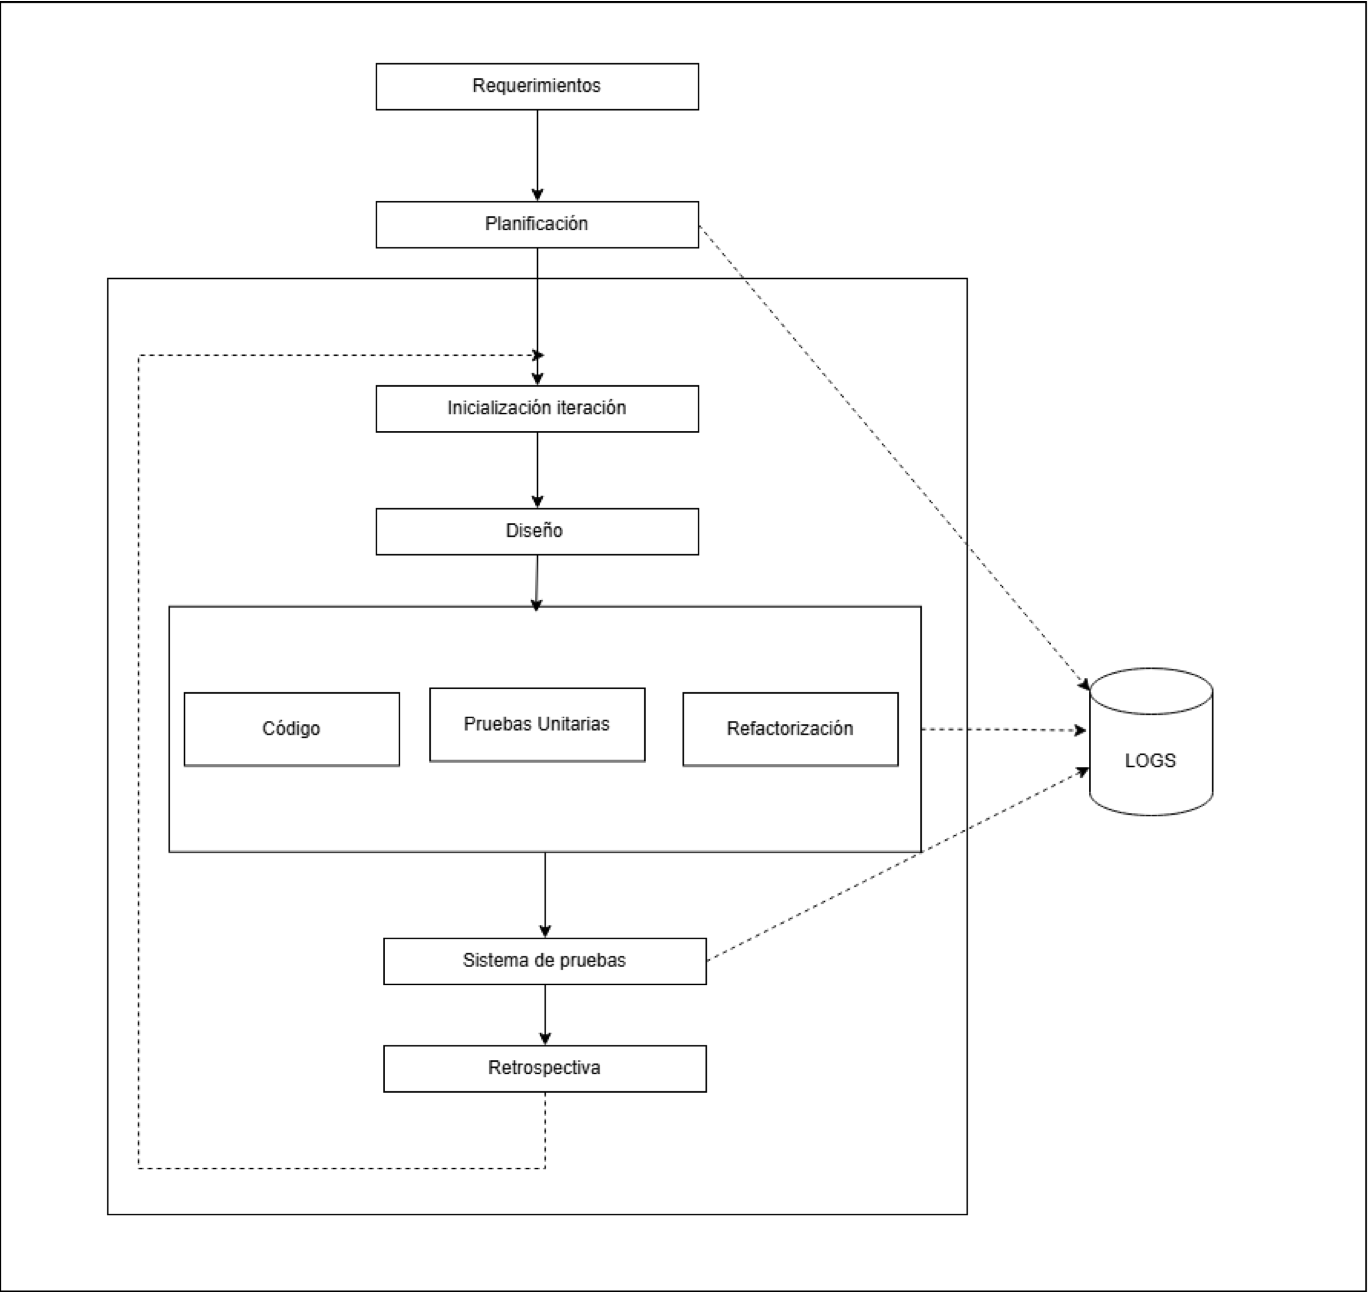
\includegraphics[width=0.8\textwidth]{fig-2-1-pxp}
  \caption[Fases de metodología Personal Extreme Programming (PXP)]{Fases de metodología Personal Extreme Programming (PXP).}
  \label{fig:pxp}
  \vspace{-2.9pt}
\end{figure}

\subsection{Metodologías de evaluación del proyecto }

En esta sección se describen las metodologías de evaluación que se implementarán para validar la calidad, usabilidad y efectividad del sistema desarrollado.

\subsubsection{Evaluación de Calidad}

Para asegurar que la plataforma esté libre de fallos críticos antes de su despliegue, se implementa una estrategia de pruebas a nivel de código y de sistema:

\begin{itemize}
  \item \textbf{Pruebas de Caja Blanca (Pruebas Unitarias y de Integración):} Estas pruebas se enfocan en verificar la lógica interna del código fuente, evaluando que los algoritmos críticos (como el motor de cálculo de cotizaciones y la lógica de proyección 3D) funcionen correctamente desde su interior. Se definen tests con el objetivo de alcanzar una cobertura de código de al menos un 95 \%.

  Para dar un ejemplo de las pruebas unitarias se considera realizar pruebas para funciones del código del programa, por ejemplo en el área de cotizaciones se ingresan valores a los insumos para verificar que los datos finales concuerden con los cálculos esperados en todo momento. A continuación, la Figura \ref{fig:cajablanca} ilustra el proceso de la prueba.

  \begin{figure}[H]
    \centering
    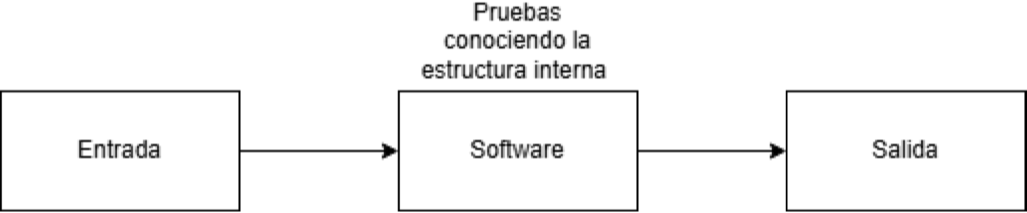
\includegraphics[width=0.6\textwidth]{fig-2-2-caja-blanca}
    \caption[Proceso de Prueba de Caja Blanca]{Proceso de Prueba de Caja Blanca.}
    \label{fig:cajablanca}
  \end{figure}

  \item \textbf{Pruebas de Caja Negra:} Corresponden a una forma de evaluar y validar el funcionamiento de los módulos del sistema sin necesidad de conocer su proceso interno. En estas pruebas, se definen entradas específicas (por ejemplo, subir un boceto y asignar horas) y se comparan con las salidas esperadas en la interfaz de usuario, garantizando que los módulos operen correctamente de extremo a extremo. A continuación, la Figura \ref{fig:cajanegra} ilustra el proceso de la prueba.

  \begin{figure}[H]
    \centering
    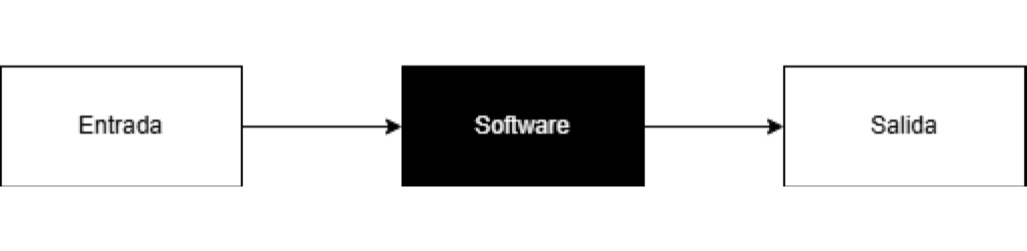
\includegraphics[width=0.6\textwidth]{fig-2-3-caja-negra}
    \caption[Proceso de Prueba de Caja Negra]{Proceso de Prueba de Caja Negra.}
    \label{fig:cajanegra}
    \vspace{9.42pt}
  \end{figure}
\end{itemize}

\subsubsection{Evaluación de Usabilidad y Aceptación}

Dado que el sistema está enfocado en usuarios finales (tatuadores y clientes del estudio), es fundamental validar que la interfaz sea intuitiva y el flujo de trabajo sea el adecuado.
\begin{itemize}
  \item \textbf{System Usability Scale (SUS)\cite{drew2018}:} Para evaluar la usabilidad empírica del sistema se considera aplicar el cuestionario estándar SUS. Este instrumento consiste en 10 afirmaciones evaluadas mediante una escala de Likert (desde ``Totalmente en desacuerdo'' hasta ``Totalmente de acuerdo''). A partir de las respuestas, se calcula un puntaje global. Para este proyecto, se ha establecido como métrica de éxito alcanzar un puntaje mínimo de 85 puntos, lo que clasificaría a la plataforma dentro de un rango de excelencia en términos de usabilidad.

  \item \textbf{Pruebas de Aceptación del Usuario (UAT)\cite{ponce}:} Se llevarán a cabo sesiones de prueba controladas donde el cliente experto y otros tatuadores invitados interactuan libremente con la versión final del sistema. Al finalizar, se registra su nivel de satisfacción, teniendo como meta alcanzar al menos un 90 \% de evaluación positiva respecto a la funcionalidad de la plataforma.
\end{itemize}

\subsubsection{Evaluación de Validación}

Para complementar las métricas de software y validar el impacto del sistema en el negocio, se considera un enfoque comparativo (Pre-test y Post-test) mediante entrevistas y análisis de registros:
\begin{itemize}
  \item \textbf{Entrevistas:} Se realiza entrevistas al inicio del proyecto para cuantificar las bases actuales del artista experto respecto a el tiempo que invierten en ajustar bocetos en papel, el tiempo que dedican a calcular costos manualmente, y su tasa de inasistencia semanal promedio.

  \item \textbf{Contraste de Resultados:} Una vez implementado el MVP y tras un periodo de prueba real, se vuelven a medir estos parámetros operando con el sistema. El objetivo es validar estadísticamente el logro en la reducción de los tiempos de previsualización en un 30 \% los tiempos de previsualización (módulo 3D), en un 40 \% los tiempos de cotización (módulo de inventario) y en un 50 \% el ausentismo (módulo de agendamiento con WhatsApp).
\end{itemize}

\section{Resumen capítulo}

En este capítulo se explicaron los conceptos básicos necesarios para entender el proyecto, se describieron las tecnologías a utilizar, evaluando alternativas y justificando la elección de cada una. También se revisó el estado del arte, presentando aplicaciones que ofrecen funcionalidades similares a la solución propuesta. Finalmente, detallaron las metodologías de desarrollo y evaluación, justificando la elección de cada una.

En el siguiente capítulo se abordará la aplicación de estas metodologías, junto con las adaptiones necesarias para el proyecto y los resultados esperados de los objetivos específicos.
